\documentclass[a4paper, 12pt]{article}

\usepackage[portuges]{babel}
\usepackage[utf8]{inputenc}
\usepackage{amsmath}
\usepackage{indentfirst}
\usepackage{graphicx}
\usepackage{multicol,lipsum}

\usepackage[hidelinks]{hyperref}   % adiciona links na TOC e nas citações

% Renomeia o título da TOC
\addto\captionsportuges{
  \renewcommand{\contentsname}
    {Sumário}
}

%%%%%%%%%%%%%%%%%%%%%%%%%%%%%%%%%%%%%%%%%%%%%%%%%%%%%%%%%%
% INÍCIO DO DOCUMENTO
%%%%%%%%%%%%%%%%%%%%%%%%%%%%%%%%%%%%%%%%%%%%%%%%%%%%%%%%%%

\begin{document}
%\maketitle

%%%%%%%%%%%%%%%%%%%%%%%%%%%%%%%%%%%%%%%%%%%%%%%%%%%%%%%%%%%
% CAPA
%%%%%%%%%%%%%%%%%%%%%%%%%%%%%%%%%%%%%%%%%%%%%%%%%%%%%%%%%%%
\begin{titlepage}
	\begin{center}
    	\begin{figure}[!ht]
        	\centering
        	
\includegraphics[width=3cm]{./imgs/uffs.png}
    	\end{figure}
    
    	\Huge{Universidade Federal da Fronteira Sul}\\
    	\large{Campus Chapecó}\\ 
    	\large{Bacharelado em Ciência da Computação}\\ 
    	
    	\vspace{15pt}
        \vspace{95pt}
        
        \textbf{\LARGE{Exercícios indicados nas aulas 05 e 06}}\\
    	
        \vspace{3,5cm}
	\end{center}
	
	\begin{flushleft}
	    \begin{tabbing}
			\textbf{Aluno:} Jean Carlo Hilger \\
			\textbf{Professor:} Andrei de Almeida Sampaio Braga \\
        \end{tabbing}
    \end{flushleft}
	
	\vspace{1cm}
	
	\begin{center}
		\vspace{\fill}
		Chapecó, março\\
		2021
	\end{center}
\end{titlepage}


%%%%%%%%%%%%%%%%%%%%%%%%%%%%%%%%%%%%%%%%%%%%%%%%%%%%%%%%%%%
% SUMÁRIO
%%%%%%%%%%%%%%%%%%%%%%%%%%%%%%%%%%%%%%%%%%%%%%%%%%%%%%%%%%%
\newpage
\tableofcontents
\thispagestyle{empty}

\newpage
\pagenumbering{arabic}

%%%%%%%%%%%%%%%%%%%%%%%%%%%%%%%%%%%%%%%%%%%%%%%%%%%%%%%%%%%
% Exercício 1
%%%%%%%%%%%%%%%%%%%%%%%%%%%%%%%%%%%%%%%%%%%%%%%%%%%%%%%%%%%
\newpage
\section{Exercício 1}


%%%%%%%%%%%%%%%%%%%%%%%%%%%%%%%%%%%%%%%%%%%%%%%%%%%%%%%%%%%
% Exercício 2
%%%%%%%%%%%%%%%%%%%%%%%%%%%%%%%%%%%%%%%%%%%%%%%%%%%%%%%%%%%
\newpage
\section{Exercício 2}

Dê a definição formal (através de uma 5-upla) dos autômatos considerados no exercício anterior.

\subsection{Autômato M1}
Definido como $(Q, \Sigma, \delta, q_s, F)$, temos:

\begin{align*}
    Q &= \{q_1, q_2, q_3\} \\
    \Sigma &= \{a, b\} \\
    \delta &= Tabela \text{\ref{tab:delta_m1}} \\
    q_s &= q_1 \\
    F &= \{q_2\}
\end{align*}

onde $\delta$ é dada pela tabela:

\begin{table}[!h]
    \centering
    \begin{tabular}{l|ll}
              & a     & b     \\ 
        \hline \hline
        $q_1$ & $q_2$ & $q_1$ \\
        $q_2$ & $q_3$ & $q_3$ \\
        $q_3$ & $q_2$ & $q_1$ \\
    \end{tabular}
    \caption{Representação da função de transição para o autômato $M_1$.}
    \label{tab:delta_m1}
\end{table}

\subsection{Autômato M2}
Definido como $(Q, \Sigma, \delta, q_s, F)$, temos:

\begin{align*}
    Q &= \{q_1, q_2, q_3, q_4\} \\
    \Sigma &= \{a, b\} \\
    \delta &= Tabela \text{\ref{tab:delta_m2}} \\
    q_s &= q_1 \\
    F &= \{q_1, q_4\}
\end{align*}

onde $\delta$ é dada pela tabela:

\begin{table}[!h]
    \centering
    \begin{tabular}{l|ll}
              & a     & b     \\ 
        \hline \hline
        $q_1$ & $q_1$ & $q_2$ \\
        $q_2$ & $q_3$ & $q_4$ \\
        $q_3$ & $q_2$ & $q_1$ \\
        $q_4$ & $q_3$ & $q_4$ \\
    \end{tabular}
    \caption{Representação da função de transição para o autômato $M_2$.}
    \label{tab:delta_m2}
\end{table}

%%%%%%%%%%%%%%%%%%%%%%%%%%%%%%%%%%%%%%%%%%%%%%%%%%%%%%%%%%%
% Exercício 3
%%%%%%%%%%%%%%%%%%%%%%%%%%%%%%%%%%%%%%%%%%%%%%%%%%%%%%%%%%%
\newpage
\section{Exercício 3}

A definição formal de um autômato finito $M$ é 
$$(\{q_1, q_2, q_3, q_4, q_5\}, \{u, d\}, \delta, q_3, \{q_3\})$$

Onde $\alpha$ é dado pela Tabela \ref{fig:table_delta} Dê o diagrama de estados desse autômato.

\begin{figure}[!ht]
    \centering
    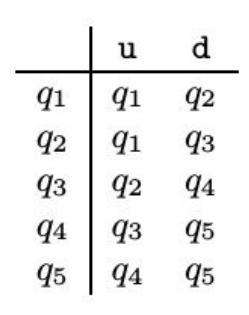
\includegraphics[width=2.6cm]{./imgs/table_delta.png}
    \caption{Tabela da função de transição $\delta$.}
    \label{fig:table_delta}
\end{figure}

\textbf{Resposta:}

\begin{figure}[ht]
    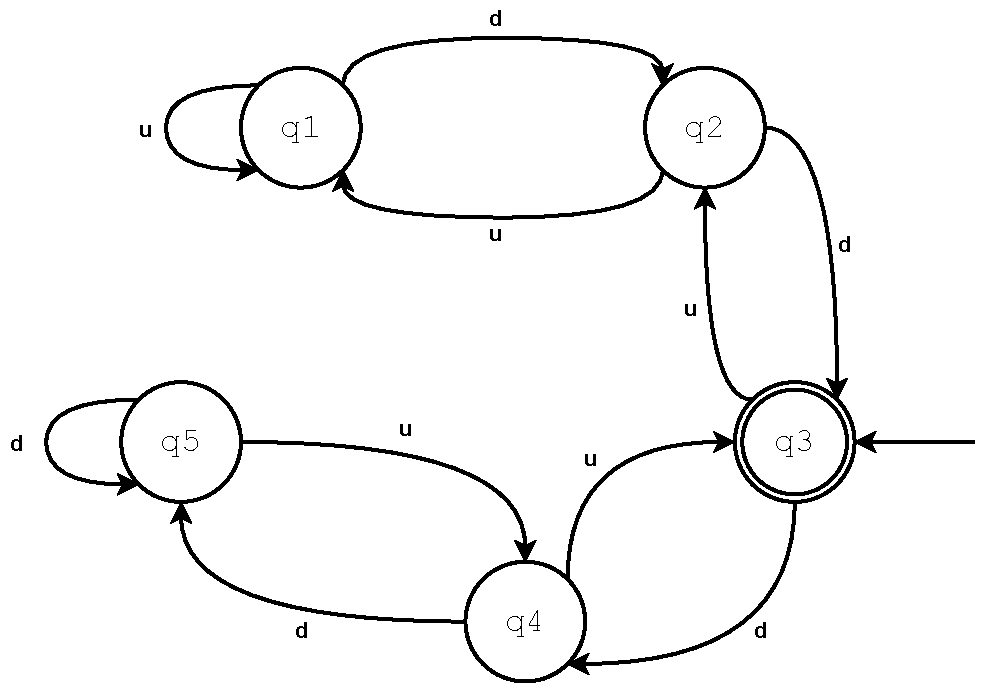
\includegraphics[width=8.4cm]{./imgs/lfa-trab-1.pdf}
    \centering
    \caption{Diagrama do autômato $M$.}
    \label{fig:diag_m}
\end{figure}

\end{document}
